\documentclass{article}

\usepackage[margin=1.5in]{geometry}
\usepackage{amsmath}
\usepackage{listings}
\usepackage{color}
\usepackage{placeins}
\usepackage{graphicx}
\graphicspath{ {/home/sajid/Desktop/Computational-Economics/Problem Set 1} }

\title{Computational Economics: Problem Set 1}
\author{S M Sajid Al Sanai}
\date{May 1, 2019}

\begin{document}

\maketitle
\pagenumbering{arabic}
\tableofcontents

\lstset{
	frame=lines,
	basicstyle=\small\sffamily,
	tabsize=4,
	columns=fixed,
	showstringspaces=false,
	showtabs=false,
	keepspaces,
	commentstyle=\color{red},
	keywordstyle=\color{blue}
}

\newpage

\section{Infinite Horizon Ramsey Model}

\subsection{Value Function Approximation}

\subsubsection{Bellman Equation}

\noindent Given our Maximisation Problem,

\begin{equation}
max_{\{ K_t \}_{t=1} ^{\infty} } \sum_{t=0} ^{\infty} \beta^t u(C_t)
\end{equation}

\noindent Where our Utility Function is specified,

\begin{equation}
u(C_t) = \ln(C_t)
\end{equation}

\noindent Where our Production Function is specified,

\begin{equation}
F(K_t) = AK^{\alpha} _t
\end{equation}

\noindent Given $K_0$ and Non-Negativity Constraints,

\begin{equation}
C_t,K_{t+1}\geq 0
\end{equation}

\noindent Given Law of Motion of Capital,

\begin{equation}
I_t=K_{t+1}-(1-\delta)K_t
\end{equation}

\noindent Given Budget Constraint limited by the Production Function,

\begin{equation}
F(K_t)\geq C_t + I_t
\end{equation}

\noindent Derive our Consumption and summarise our Production,

\begin{equation}
C_t = F(K_t)-K_{t+1}+(1-\delta)K_t
\end{equation}

\begin{equation}
f(K_t) = F(K_t)+(1-\delta)K_t
\end{equation}

\begin{equation}
\implies C_t=f(K_t)-K_{t+1}
\end{equation}

\noindent Substituting Consumption into our Maximisation Problem allows us to derive our Bellman Equation,

\begin{equation}
V( K_t ) = max_{ \{ K_{t+1} \} } u( f(K_t) - K_{t+1} ) + \beta V(K_{t+1})
\end{equation}

\begin{equation}
V( K_t ) = max_{ \{ K_{t+1} \} } \ln( AK^{\alpha} _t - (1-\delta)K_t - K_{t+1} ) + \beta V(K_{t+1})
\end{equation}

\newpage

\subsubsection{Value Function Iteration}

Value Function Iteration conducted over the discretised space for Capital assuming $\beta=0.6, \ A=20, \ \alpha=0.3,$ and $\delta=0.5$ yields the following graph visualising output,

\begin{figure}[h]
\begin{center}
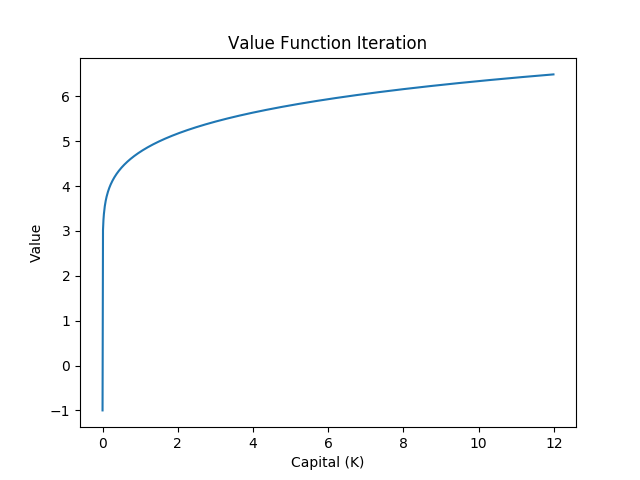
\includegraphics[width=\textwidth]{Figure1.png}
\caption{Value Function Iteration over Discretised Capital}
\end{center}
\end{figure}
\FloatBarrier

\newpage

\subsection{Customised Value Function Approximation}

\subsubsection{Using Iteration}

Value Function Iteration conducted over the discretised space for Capital assuming $\beta=0.6, \ A=1, \ \alpha=0.3,$ and $\delta=1$ yields the following graph visualising output,

\begin{figure}[h]
\begin{center}
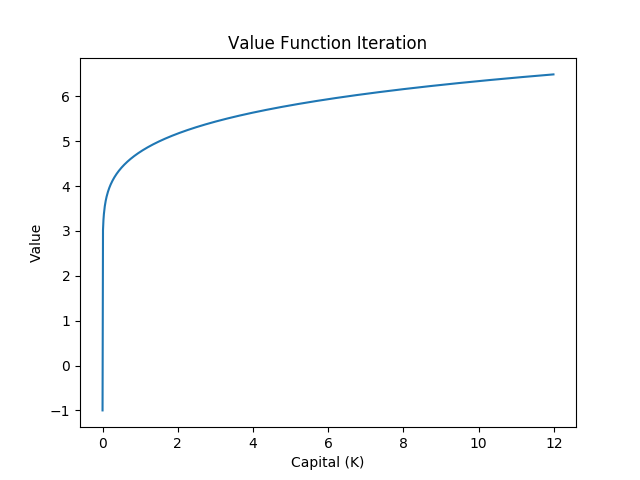
\includegraphics[width=\textwidth]{Figure1.png}
\caption{Value Function Iteration over Discretised Capital}
\end{center}
\end{figure}
\FloatBarrier

\newpage

\subsubsection{Using Analytical Form}

Value Function Iteration conducted over the discretised space for Capital assuming $\beta=0.6, \ A=1, \ \alpha=0.3,$ and $\delta=1$ is superimposed with the Analytical Form for comparison of output,

\begin{figure}[h]
\begin{center}
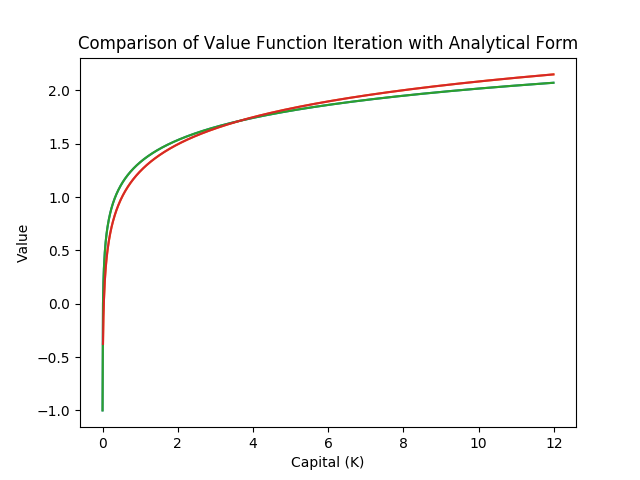
\includegraphics[width=\textwidth]{Figure3.png}
\caption{Comparison of Value Function Iteration with Analytical Form}
\end{center}
\end{figure}
\FloatBarrier

With our initial guess of the functional form of the analytical form being,

\begin{equation}
V(K_t) = A + B \ln K_t
\end{equation}

\begin{equation}
\implies A = \frac{\alpha \beta}{1- \alpha \beta} \ln \alpha \beta
\end{equation}

\begin{equation}
\implies B=\frac{\alpha}{1-\alpha\beta}
\end{equation}

\newpage

\section{Rust Model}

\subsection{Maximum Likelihood Estimator}

The Maximum Likelihood Estimator for $\lambda$ is described below, where $S$ is the number of state transitions and $T$ is the time periods of simulation.

$$\lambda_{MLE} = \frac{J}{T}$$

\subsection{Value Function Iteration}

\subsubsection{Choice Specific Value Function}

\begin{figure}[h]
\begin{center}
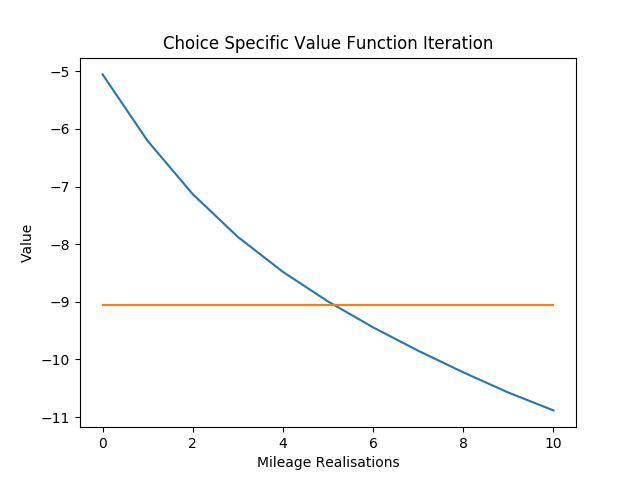
\includegraphics[width=\textwidth]{Figure4.png}
\caption{Value Functions for Replacement Decisions}
\end{center}
\end{figure}
\FloatBarrier

\newpage

% Code Snippet
\begin{lstlisting}
[[ V0; V1 ]]
[[ -5.0550212   -9.0550212 ]
 [ -6.2082666   -9.0550212 ]
 [ -7.13225472  -9.0550212 ]
 [ -7.87342411  -9.0550212 ]
 [ -8.4803681   -9.0550212 ]
 [ -8.99362596  -9.0550212 ]
 [ -9.44281035  -9.0550212 ]
 [ -9.84815671  -9.0550212 ]
 [-10.22296267  -9.0550212 ]
 [-10.57401037  -9.0550212 ]
 [-10.88331338  -9.0550212 ]]
\end{lstlisting}

% Code Snippet
\begin{lstlisting}
Conditional Choice Probabilities:
[[ x; Pr(i=0|x,theta); Pr(i=1|x,theta); ]]
[[ 0.          0.98201379  0.01798621]
 [ 1.          0.94515068  0.05484932]
 [ 2.          0.87244661  0.12755339]
 [ 3.          0.76523484  0.23476516]
 [ 4.          0.63983616  0.36016384]
 [ 5.          0.51534399  0.48465601]
 [ 6.          0.40424963  0.59575037]
 [ 7.          0.31149581  0.68850419]
 [ 8.          0.23722727  0.76277273]
 [ 9.          0.17961042  0.82038958]
 [10.          0.13844185  0.86155815]]
\end{lstlisting}

\newpage

\subsubsection{Integrated Value Function}

\begin{figure}[h]
\begin{center}
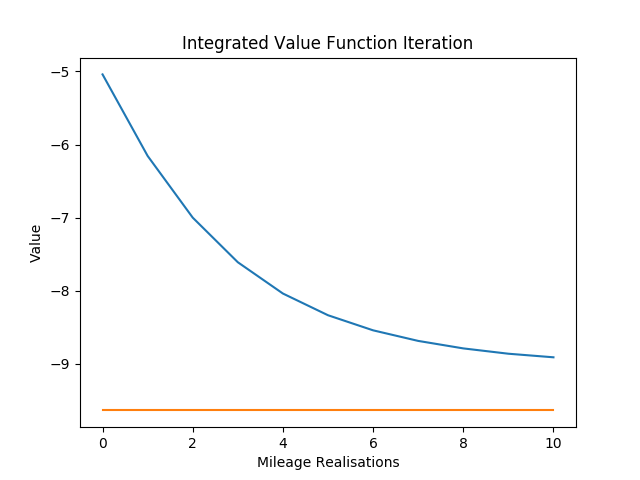
\includegraphics[width=\textwidth]{Figure5.png}
\caption{Value Functions for Replacement Decisions}
\end{center}
\end{figure}
\FloatBarrier

% Code Snippet
\begin{lstlisting}
[[ V0; V1 ]]
[[-5.04076462]
 [-6.15574904]
 [-6.99969426]
 [-7.60974496]
 [-8.03771832]
 [-8.33459865]
 [-8.54098101]
 [-8.68568068]
 [-8.78811939]
 [-8.8609386 ]
 [-8.90990183]]
\end{lstlisting}

\newpage

% Code Snippet
\begin{lstlisting}
Conditional Choice Probabilities:
[[ x; Pr(i=0|x,theta); Pr(i=1|x,theta); ]]
[[ 0.          0.98201379  0.01798621]
 [ 1.          0.94515068  0.05484932]
 [ 2.          0.87244661  0.12755339]
 [ 3.          0.76523484  0.23476516]
 [ 4.          0.63983616  0.36016384]
 [ 5.          0.51534399  0.48465601]
 [ 6.          0.40424963  0.59575037]
 [ 7.          0.31149581  0.68850419]
 [ 8.          0.23722727  0.76277273]
 [ 9.          0.17961042  0.82038958]
 [10.          0.13844185  0.86155815]]
\end{lstlisting}

\subsubsection{Comparison of Value Function Iterations}

\begin{figure}[h]
\begin{center}
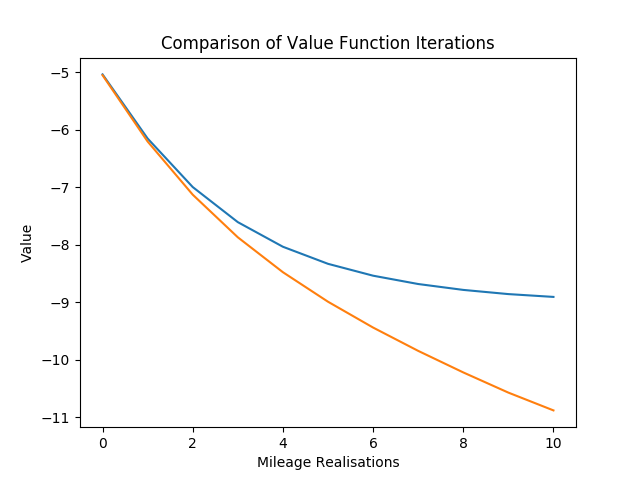
\includegraphics[width=\textwidth]{Figure6.png}
\caption{Simulated Frequencies of Replacement Decisions}
\end{center}
\end{figure}
\FloatBarrier

\newpage

\subsection{Forward Simulation}

Forward Simulation was conducted over $T=5000$ periods using pre-defined parameters.

\begin{figure}[h]
\begin{center}
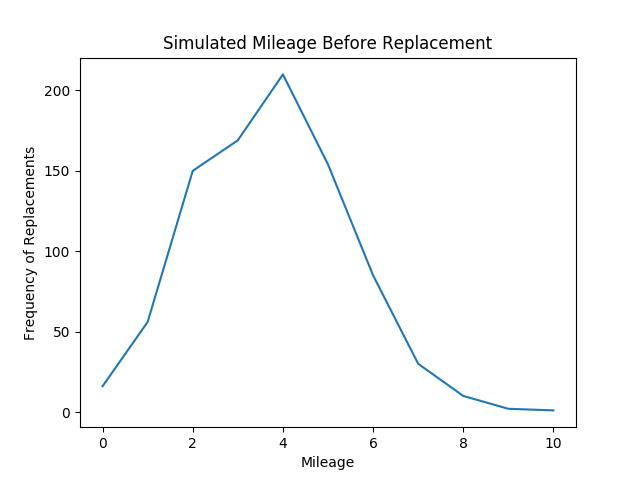
\includegraphics[width=\textwidth]{Figure7.png}
\caption{Simulated Frequencies of Replacement Decisions}
\end{center}
\end{figure}
\FloatBarrier

\begin{figure}[h]
\begin{center}
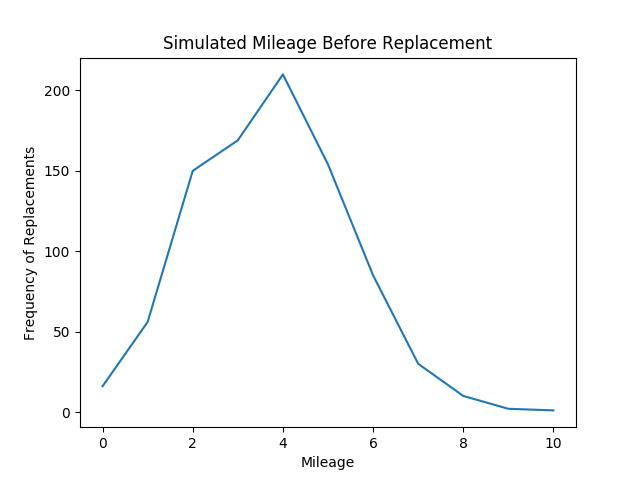
\includegraphics[width=\textwidth]{Figure8.png}
\caption{Simulated Mileage before Replacement}
\end{center}
\end{figure}
\FloatBarrier

\subsection{Maximum Likelihood Estimation}

Given an initial guess for $\theta = \big( 0.3, 0, 4 \big)$, use of the Nested Fixed Point Algorithm yields the minimised $\theta = \big( 0.82498424, -0.03871543,  2.14309007 \big)$ as shown below.

% Code Snippet
\begin{lstlisting}
Minimised Theta:
      fun: 5319.407700566876
 hess_inv: array([[ 4.16487948e-08, -9.90443077e-10, -1.04954367e-07],
       [-9.90443077e-10,  2.32738993e-10,  3.50993346e-09],
       [-1.04954367e-07,  3.50993346e-09,  2.71644050e-07]])
      jac: array([ 0.00787354, -0.00042725,  0.00372314])
  message: 'Desired error not necessarily achieved due to precision loss.'
     nfev: 595
      nit: 19
     njev: 115
   status: 2
  success: False
        x: array([ 0.82498424, -0.03871543,  2.14309007])
\end{lstlisting}

\subsection{Forward Simulation with Minimised Parameters}

\subsubsection{Long Run Replacement Probabilities}

Forward Simulation was conducted over $T=5000$ periods using minimised parameters.

% Code Snippet
\begin{lstlisting}
Conditional Choice Probabilities:
[[ x; Pr(i=0|x,theta); Pr(i=1|x,theta); ]]
[[0.00000000e+00 6.40422872e-01 3.59577128e-01]
 [1.00000000e+00 1.40895563e-01 8.59104437e-01]
 [2.00000000e+00 2.67150030e-04 9.99732850e-01]
 [3.00000000e+00 6.16598042e-09 9.99999994e-01]
 [4.00000000e+00 1.95745003e-15 1.00000000e+00]
 [5.00000000e+00 8.54899058e-24 1.00000000e+00]
 [6.00000000e+00 5.13658649e-34 1.00000000e+00]
 [7.00000000e+00 4.24590219e-46 1.00000000e+00]
 [8.00000000e+00 4.82837483e-60 1.00000000e+00]
 [9.00000000e+00 7.55383654e-76 1.00000000e+00]
 [1.00000000e+01 1.62581004e-93 1.00000000e+00]]
\end{lstlisting}

% Code Snippet
\begin{lstlisting}
Long Run Replacement Probabilities:
 [[ x; Pr(i=0|x,theta); Pr(i=1|x,theta); ]]
[[ 0.          0.64866582  0.35133418]
 [ 1.          0.12943262  0.87056738]
 [ 2.          0.          1.        ]
 [ 3.                 nan         nan]
 [ 4.                 nan         nan]
 [ 5.                 nan         nan]
 [ 6.                 nan         nan]
 [ 7.                 nan         nan]
 [ 8.                 nan         nan]
 [ 9.                 nan         nan]
 [10.                 nan         nan]]
\end{lstlisting}

\begin{figure}[h]
\begin{center}
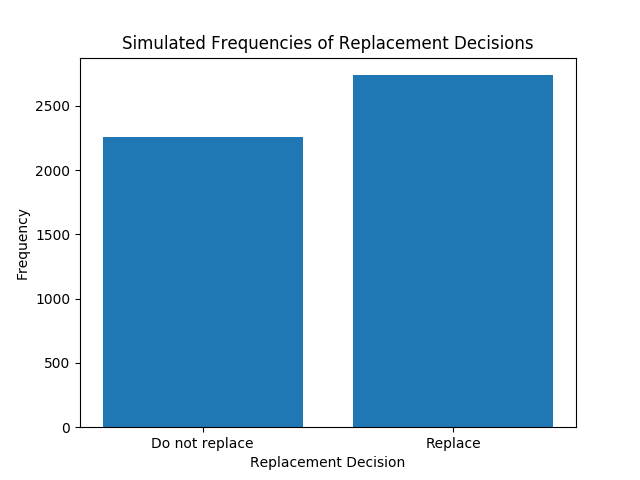
\includegraphics[width=\textwidth]{Figure9.png}
\caption{Simulated Frequencies of Replacement Decisions}
\end{center}
\end{figure}
\FloatBarrier

\begin{figure}[h]
\begin{center}
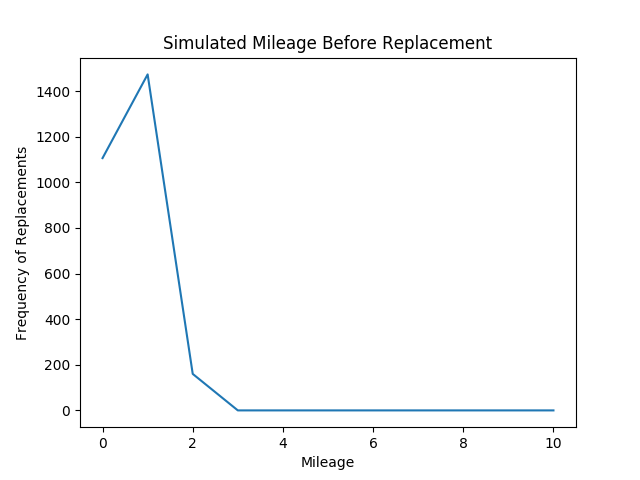
\includegraphics[width=\textwidth]{Figure10.png}
\caption{Simulated Mileage before Replacement}
\end{center}
\end{figure}
\FloatBarrier

\subsubsection{Long Run Replacement Probabilities (SS)}

Forward Simulation was conducted over $T=5000$ periods using minimised parameters.

% Code Snippet
\begin{lstlisting}
(Comparative) Long Run Replacement Probabilities:
[[ x; Pr(i=0|x,theta); Pr(i=1|x,theta); ]]
[[0.00000000e+00 9.47343641e-01 5.26563593e-02]
 [1.00000000e+00 7.40359258e-01 2.59640742e-01]
 [2.00000000e+00 7.62908025e-01 2.37091975e-01]
 [3.00000000e+00 8.06716979e-01 1.93283021e-01]
 [4.00000000e+00 8.66584961e-01 1.33415039e-01]
 [5.00000000e+00 9.25288440e-01 7.47115598e-02]
 [6.00000000e+00 9.66831443e-01 3.31685572e-02]
 [7.00000000e+00 9.88319617e-01 1.16803827e-02]
 [8.00000000e+00 9.96664368e-01 3.33563219e-03]
 [9.00000000e+00 9.99197164e-01 8.02835743e-04]
 [1.00000000e+01 9.99786104e-01 2.13896282e-04]]
\end{lstlisting}

\subsubsection{Counterfactual with Subsidy on Minimised Parameters}

Forward Simulation was conducted over $T=5000$ periods using minimised parameters with an additional $10$\% subsidy. Differentials were obtained with Long Run Replacement Probabilities obtained on minimised parameters prior to application of subsidy.

% Code Snippet
\begin{lstlisting}
(10% Subsidy) Long Run Replacement Probabilities:
[[ x; Pr(i=0|x,theta); Pr(i=1|x,theta); ]]
[[ 0.          0.88235294  0.11764706]
 [ 1.          0.63238771  0.36761229]
 [ 2.          0.37897043  0.62102957]
 [ 3.          0.19230769  0.80769231]
 [ 4.          0.12765957  0.87234043]
 [ 5.          0.25        0.75      ]
 [ 6.          0.          1.        ]
 [ 7.                 nan         nan]
 [ 8.                 nan         nan]
 [ 9.                 nan         nan]
 [10.                 nan         nan]]
\end{lstlisting}

% Code Snippet
\begin{lstlisting}
(Differential) Long Run Replacement Probabilities:
[[ x; Pr(i=0|x,theta); Pr(i=1|x,theta); ]]
[[ 0.         -0.23368712]
 [ 1.         -0.50295508]
 [ 2.         -0.37897043]
 [ 3.                 nan]
 [ 4.                 nan]
 [ 5.                 nan]
 [ 6.                 nan]
 [ 7.                 nan]
 [ 8.                 nan]
 [ 9.                 nan]
 [10.                 nan]]
\end{lstlisting}

\newpage

\section{Appendix}

\subsection{Source}

\subsubsection{Source: Question 1}

\lstinputlisting[language=Python]{pset1_1_source.py}

\newpage

\subsubsection{Source: Question 2}

\lstinputlisting[language=Python]{pset1_2_source.py}

\newpage

\subsection{Output}

\lstinputlisting{pset1_output.txt}

\end{document}